\chapter{Implementace}

\section{Vue.js framework}
Klientská část aplikace je postavena nad Vue.js frameworkem, jež je populární JavaScriptový framework na stavbu uživatelských rozhraní. Protože některé z jeho funkcionalit byly použity v klíčových částech aplikace, je nutné čtenáře obeznámit alespoň se základním principem fungování frameworku.

\subsection{Vuex}
Vue.js framework, podobně jako konkurenční React\footnote{\url{https://reactjs.org/}} (Facebook) nebo Angular\footnote{\url{https://angularjs.org/}} (Google), využívají principu sledování stavu aplikace (jejich dat) pro automatickou změnu DOMu webové stránky. V praxi to znamená, že programátor může velice snadno napsat kód, který generuje uživatelské rozhraní na základě dat, která mohou být libovolně měněna bez nutnosti řešit problém, zda ke změně vůbec došlo a které části aplikace mají být o změně stavu informovány. Ve Vue tuto funkcionalitu zastává právě Vuex\footnote{\url{https://vuex.vuejs.org/}}, jež je možný používat samostatně.

Vuex drží stav aplikace jako jeden objekt (tedy slouží jako centrální úložiště dat pro celou aplikaci). Tento objekt se nazývá \textbf{store}. Změny ve storu mohou být sledovány Vuexem pro vykonání libovolných akcí, například překreslení textu na stránce, jež byl vykreslen Vue frameworkem.

\newcommand{\inlinecode}{\texttt}

Vrátíme-li se k původnímu příkladu, programátorovi stačí přiřadit do proměnné, jež je spravovaná Vuexem, novou hodnotu a Vuex se postará o zavolání všech komponent, které tuto proměnnou využívají a tyto komponenty na stránce překreslí původní hodnotu na novou. Překreslení přitom proběhne až poté, co skončí průběh aktuální funkce. Tohoto je docíleno pomocí \\  \texttt{Window.requestAnimationFrame()}. Díky tomuto můžeme stav v rámci průběhu jedné funkce modifikovat vícekrát se skoro nulovým dopadem na celkový výkon aplikace.

\subsubsection{Computed properties}

Kromě této funkcionality Vuex nabízí takzvané \textbf{gettery}, jež jsou ve Vue frameworku nazývány jako \textbf{computed properties}. Jedná se o funkce, které využívají data ze storu pro výpočet dat nových. Výhoda takovýchto getterů je ta, že Vuex dokáže výsledky těchto funkcí cachovat a přepočítává je pouze tehdy, změní-li se data původní. Interně gettery fungují tak, že při zavolání klientské funkce Vuex sleduje které části storu byly dotázany a ty pak sleduje na změnu jež invaliduje cache konkrétního getteru. Při příštím požadavku na hodnotu se pak klientská funkce volá znovu a celá operace se opakuje.

Tyto computed properties jsou v aplikaci využívány často. Kupříkladu funkce, která počítá, zda je sousední uzel vybrán. Na takovouto hodnotu se v aplikaci mohu ptát libovolně krát, ale počítá se pouze tehdy, když se množina sousedních uzlů vrcholu změní, nebo se změní právě označení uzlu z množiny.

\subsubsection{Watchers}

Ve Vue lze využívat i \textbf{watch}ery, které umožňují registraci callbacku na změnu určité proměnné ve stavu. Watchery má smysl využívat tam, kde již data přestávají být spravována Vue frameworkem, tedy u knihoven třetích stran. Watchery, podobně jako překreslení komponent, jsou volány až po skončení probíhající funkce.

\subsubsection{Změna stavu}

Jak již bylo zmíněno, stav lze měnit přiřazením do proměnné, popřípadě voláním metod jako \texttt{.push()} na poli. Vuex dokáže tyto změny sledovat nahrazením původní proměnné (máme na mysli položku objektu) JavaScriptovým setterem. U polí dojde k obalení metody \texttt{.push()} jež registruje změnu stavu.

Tento přístup má několik nevýhod, které se promítly i při vývoji klientské aplikace:
\begin{itemize}
  \item Vue není plně kompatibilní s novými \textbf{ES6 kontejnery} \texttt{Map} a \texttt{Set} a proto jsou v aplikaci používány jen v rámci lokálních proměnných a mapa je nahrazena klasickým objektem.
  \item Protože je v JavaScriptu nemožné sledovat \textbf{vytvoření nové property objektu}, musí programátor v tomto případě volat ručně \texttt{Vue.set(target, propertyName/index, value)} a \texttt{Vue.delete}, popřípadě vytvořit nový objekt který nahradí ten původní.
  \item Je důležité mít na paměti, že data ve storu již nejsou původními objekty v pravém slova smyslu, ale veškeré fieldy a metody u polí byly nahrazeny, jak je zmíněno výše. Proto předání objektů a polí ze storu knihovnám třetích stran je nutné ošetřit \textbf{oklonováním objektu}, jinak může dojít k zaseknutí aplikace.
  \item Instance tříd \textbf{knihoven třetích stran může zaseknout aplikaci}, pokud ji uložíme do storu. Bohužel, tohoto je velmi snadné ve Vue frameworku dosáhnout omylem. Problém je rozebrán v následující kapitole.
\end{itemize}

\subsection{Vue framework}
Vue framework využívá takzvané komponenty. Komponentou se rozumí prvek na stránce se kterým má smysl pracovat samostatně. Každá komponenta má vlastní HTML, CSS a JS. Komponenty se mohou do sebe zanořovat a vytvářet tak větší komponenty z menších. Příkladem může být komponenta \textit{seznam} jež dokáže na stránku vykreslit senznam prvků. Takováto komponenta by pak mohla mít podkomponenty jako \textit{prvek seznamu}.

Každé komponentě lze předat data formou \textbf{properties} přičemž komponenta na základě těchto dat může vyrobit pod sebou další komponenty a předat jim část dat, která dostala.

Tyto předávána data jsou právě data ze storu. Vue framework doporučuje, aby data co koponenta dostane formou properties neupravovala přímo, ale místo toho posílala události rodičovské komponentě, která data upraví. Ve své práci jsem se \textbf{rozhodl toto doporučení ignorovat}, neboť by tímto vzrostla náročnočnost na správu aplikace.

\begin{figure}[h]
    \centering
    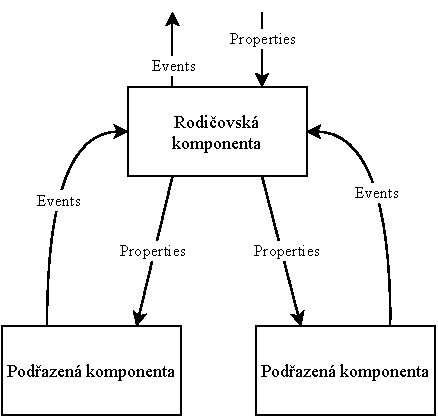
\includegraphics[width=0.5\textwidth]{media/vue.pdf}
    \caption{Doporučený způsob komunikace mezi komponentami ve Vue frameworku}
\end{figure}

\subsection{Loaders}
Kód Vue komponent se zapisuje do souborů s příponou \texttt{.vue}. Při sestavování aplikace se pak použije \texttt{vue-loader} který ze souboru vyextrahuje zvlášť CSS, JS a HTML a ty předá dál na zpracování. HTML kód komponent není ve skutečnosti pravý HTML. Jedná se nadstavbu umožňující psát speciální značky, jež rozhodují kolikrát a jestli vůbec se tag na stránce vyrenderuje. Tato HTML nadstavba je pak předána \texttt{vue-template-compiler} který vyrobí optimalizovaný JS kód jež renderuje HTML na základě stavu komponenty.

\newpage

\begin{prikl}
Ukázka jednoduché Vue komponenty \texttt{IndexedList} která má parametr \texttt{list} očekávající pole stringů. Tato komponenta vypíše pole v odrážkovém seznamu ve formě \texttt{index: hodnota}. Komponenta se sama stará o překreslení DOMu, když se změní data. Komponentu můžeme v jiné komponentě použít vložením \texttt{<indexed-list :list="inputData" />} kde \texttt{inputData} je proměnná obsahující pole stringů.

\begin{code}
<template>
  <ul>
    <li v-for="(item, index) in list" :key="index">
      {{index}}: {{ item }}
    </li>
  </ul>
</template>

<script lang="ts">
  import {Component, Prop} from "vue-property-decorator";
  import Vue from "vue";
  @Component
  export default class IndexedList extends Vue {
    @Prop() private list: string[];
  }
</script>

<style scoped lang="scss">
  ul {
    color: red;
  }
</style>
\end{code}
\end{prikl}

\subsubsection*{Scoped styly}

Můžeme si povšimnout \texttt{scoped} stylů v ukázce. Vue má mechanismus, že styly které zde nastavíme se aplikují jen na tuto komponentu. Nastavením červené barvy na seznam jsme tedy skutečně nastavili červenou barvu jen této komponentě a ostatní seznamy jsou netknuté. Toto má nespornou výhodu pokud pracujeme s velkým množstvím komponent a hrozilo by, že bychom museli používat složitě pojmenované css třídy aby nedošlo ke kolizi.

Pokud bychom chtěli ovlivnit styly vnořených komponent a máme nastavené scoped styly, musíme použít pseudoselektor \texttt{::v-deep}, kupříkladu \\  \texttt{.actions ::v-deep .v-input--selection-controls}. Tohoto je hodně používáno poukud je potřeba upravit styly Vuetify frameworku (viz dále).

\newpage

\section{Programátorská dokumentace}
V této sekci budou postupně rozebrány klíčové třídy a komponenty aplikace.

\subsection{Vstupní skript a pomocné soubory}
Vstupním skriptem celé aplikace je soubor \texttt{main.ts} ve kterém je inicializován Vuetify a Vue framework, který spouští komponentu Application, jež je výchozí komponentou celé aplikace.

V tomto souboru je také includován soubor \texttt{LiteralTranslator.ts} který přidává pomocné globální metody (v rámci Vue frameworku jsou dostupné pod \texttt{this}) pro překlad literálů z grafu.

\begin{itemize}
  \item \texttt{\$t_literal(translations): string|undefined} - Očekává objekt \\popsaný v kapitole \ref{jazykova-podpora} a vybere z něj nejvhodnější překlad podle pravidel popsaných ve zmíněné kapitole. Vrací \texttt{undefined} pokud žádný překlad není.

  \item \texttt{\$te_literal(translations): boolean} - Vrací true, pokud by předchozí metoda našla překlad.

  \item \texttt{\$i18nGetAllLanguages(): string[]} - Vrací jazyky které jsou požadovány ze serveru. Pokud se jazyk aplikace změní a na již stažená data vrátí \texttt{\$te_literal} false, pak se data stáhnou znovu s již správným jazykem. Tato logika je zatím implementována pouze u meta konfigurací a konfigurací.
\end{itemize}

\subsection{Komponenta Application}
Jedná se kořenovou komponentu celé aplikace, která drží základní třídy a moduly a řídí logiku celé aplikace. Tato komponenta registruje veškeré dialogové okna a grafické prvky.

Pro debugování aplikace je komponenta přístupná pod \texttt{window.kgwb} a je tedy možné zasahovat do jakékoli části aplikace.

Mezi důležité fieldy patří (veškeré tyto třídy budou popsány dále v textu):
\begin{itemize}
  \item \texttt{server: RemoteServer} - Třída komunikující se serverem. Obsahuje metody které zavolají na serveru konkrétní požadavek a vrátí výsledek ve správném interface nebo false, pokud nastala chyba.
  \item \texttt{configuration: Configuration} - Aktuální konfigurace grafu ve smyslu konfigurace z kapitoly \ref{pozadavky-konfigurace}.
  \item \texttt{graph: Graph} - Aktuální graf jež závisí na \texttt{configuration}.
  \item \texttt{areaManipulator: GraphAreaManipulator} - Třída která obsahuje \\ metody pro práci s grafovou oblastí jako zoomování, přesouvání pohledu atp.
  \item \texttt{manipulator: GraphManipulator} - Třída která obsahuje metody pro složitější práci s grafem. Na rozdíl od \texttt{Graph} metody v této třídě více odpovídají akcím uživatele a obvykle volají další moduly jako \texttt{LayoutManager}.
  \item \texttt{viewOptions: ViewOptions} - Jednoduchá třída mající stav, jak pohlížet na graf. Řeší zda u hran mají být popisky a zda vůbec mají být hrany viditelné. U vrcholů pak řeší také viditelnost popisků a zda se mají zobrazit jako malé tečky.
  \item \texttt{filter: FiltersList} - Modul řešící filtrování.
  \item \texttt{layouts: LayoutManager} - Modul řešící layoutování grafu v závislosti na určitých akcích uživatele.
  \item \texttt{configurationManager: ConfigurationManager} - Drží všecny načtené konfigurace a metakonfigurace ze serveru.
  \item \texttt{visualStyleSheet: ResponseStylesheet} - Aktuální stylesheet pro \\ Cytoscape knihovnu.
  \item \texttt{graphSearcher: GraphSearcher} - Třída schopna vyhledávat vrcholy v grafu a z autocomplete souborů jež jsou specifikovány v konfiguraci.
\end{itemize}

\subsubsection{Závislost modulů}

Značná část modulů v aplikaci je závislá na jiných. Kupříkladu \texttt{Graph} je závislý na \texttt{RemoteServer} a částečně na \texttt{Configuration}. Na třídě \texttt{Graph} pak závisí \texttt{GraphAreaManipulator} na které závisí \texttt{GraphManipulator}. Protože těchto závislostí je hodně, některé třídy byly určeny jako readonly a tedy se může měnit pouze jejich stav. Jedná se například o třídu \texttt{RemoteServer} které lze měnit URL adresu serveru. Dalšími třídami jsou \texttt{GraphAreaManipulator}, \texttt{ViewOptions}, \texttt{FiltersList}, \texttt{LayoutManager}, \texttt{ConfigurationManager}. Ostaní třídy jsou pak měněny pouze když se mění konfigurace, v tu chvíli se starý graf zahazuje a vytváří se nový.

\medskip

Mezi důležité metody patří
\begin{itemize}
  \item \texttt{async loadStylesheet()} - Načte stylesheet do proměnné \\ \texttt{visualStyleSheet} podle aktuální konfigurace \texttt{configuration}.
  \item \texttt{changeConfiguration()} - Nastaví novou konfiguraci \texttt{configuration} a zavolá metodu \texttt{createNewGraph}.
  \item \texttt{createNewGraph(loadStylesheet: boolean = true)} - Na základě konfigurace \texttt{configuration} vytvoří nový, prázdný graf (startý zahodí) a nastaví závislosti mezi moduly. Tato metoda pak ještě resetuje nastavení filtrů a plátna kde se vykresluje graf.
  \item \texttt{updateGraphSearcher()} - Pomocná metoda pro \texttt{createNewGraph} která na základě konfigurace a grafu sestaví třídu schopnou vyhledávat nové vrcholy v grafu.
\end{itemize}

Kromě těchto metod komponenta obsahuje ještě Vue metodu \texttt{mounted} která skryje uvítací obrazovku aplikace až se komponenta (a tedy i celá aplikace) inicializuje. Kontroluje také URL adresu, zda neobsahuje parametry \texttt{load}, \\ \texttt{meta-configuration} nebo \texttt{configuration} které přimějí aplikaci načíst graf z url respektive načíst meta konfiguraci respektive konfiguraci.

\subsubsection{ApplicationLoadStoreMixin}
\texttt{ApplicationLoadStoreMixin} rozšiřuje komponentu o načítání a ukládání grafu ze a do souboru.

\paragraph{askForSaveAndPerformAction(modal: boolean, callback: Function)}\mbox{}\\ Tato funkce zkontroluje, zda jsou v grafu nějaké neuložené změny a pokud ano, otevře \texttt{SaveDialog} komponentu. Podle odpovědi na dialog pak graf uloží a v případě kladného potvrzení zavolá \texttt{callback} funkci která pak může například vytvořit nový graf. Pokud žádné změny nejsou, callback je volán okamžitě.

\paragraph{loadFromFile(file: File), loadFromUrl(url: string)} - Metoda otevře soubor respektive soubor z URL a přečte ho jako JSON. Výsledný objekt pak předá metodě \texttt{ObjectSave::restoreFromObject}.

\paragraph{saveToFile()} - Vyrobí soubor se stavem aplikace který je možné stáhnout.

\subsection{Interface file-save/ObjectSave}
Interface \texttt{ObjectSave} předepisuje dvě metody \texttt{saveToObject(): object} a \texttt{restoreFromObject(object: any): void} které uloží stav třídy do serializovatelného objektu, respektive tento stav obnoví. Tento interface obsahují všechny třídy jež drží stav aplikace který je třeba uložit do souboru, pokud o to uřivatel požádá.

Tento interface implemetuje i komponenta \texttt{Application} jež tyto metody volá na modulech a jednotlivé výsledky pak spojí do jednoho objektu (v případě metody \texttt{saveToObject}). Výsledek je pak serializován do JSONu a uložen do počítače. V opačném případě je JSON deserializován a předán metodě \texttt{restoreFromObject} která volá tuto metodu na modulech které ji mohou volat na podtřídách.

\paragraph{Poznámka:} Je třeba mít na paměti, že metoda \texttt{saveToObject} by měla vracet plain Javascript objekt, tedy veškeré neprimitivní typy jako objekty a pole musí být oklonovány, pokud jsou ve vlastnictví Vue frameworku. Taktéž je třeba dbát na zpětnou kompatibilitu u metody \texttt{restoreFromObject}.

\smallskip

Do budoucna se nabízí tento interface rozšířit o více módů ukládání. Tento problém je popsán v poslední kapitole.

\subsection{Třída Graph}

\begin{figure}
    \centering
    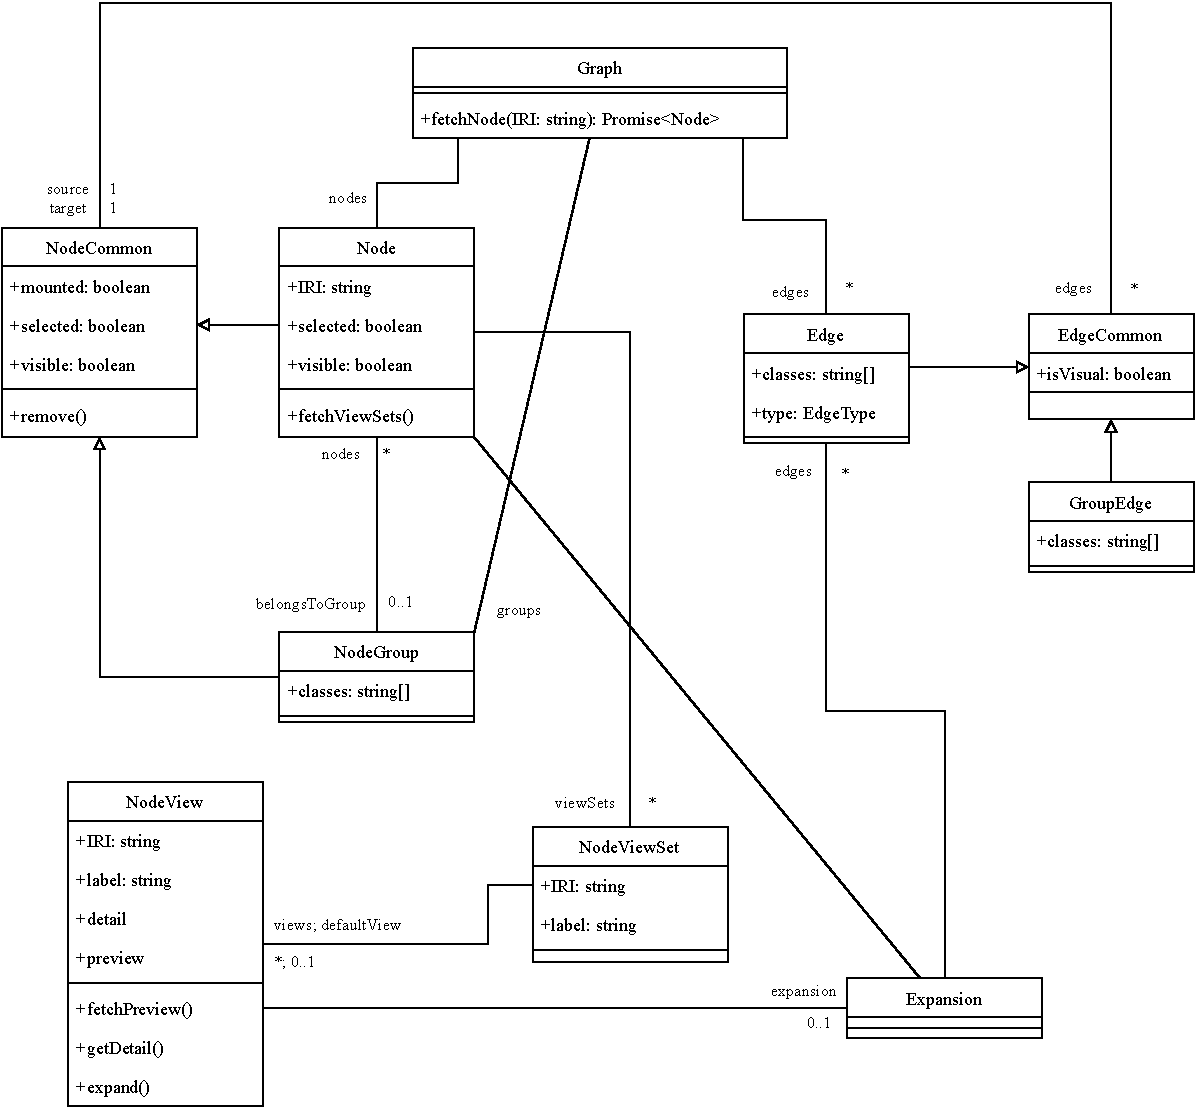
\includegraphics[width=\textwidth]{media/graph.pdf}
    \caption{Class diagram části aplikace jež pracuje s grafem.}
\end{figure}

Třída \texttt{Graph} umístěna v \texttt{graph/} spravuje stažený graf pod konkrétní konfigurací. Závisí na \texttt{server: RemoteServer} a \texttt{configuration: Configuration}. Pokud se konfigurace mění, nebo se načítá nový graf ze souboru, je tato třída zahozena. Ačkoli třídy jako \texttt{Node} nebo \texttt{Edge} obsahují fieldy pro obsluhu viditelného grafu, třída \texttt{Graph} a ostatní nemusí být explicitně použity na vykreslení grafu na plátno, ale mohou být použity pro držení obecného grafu.

\subsubsection*{Fieldy}
\begin{itemize}
  \item \texttt{nodes} objekt tříd \texttt{Node} - Seznam všech vrcholů grafu.
  \item \texttt{edges} objekt tříd \texttt{Edge} - Seznam všech hran stažených ze serveru.
  \item \texttt{groups: NodeGroup[]} - Seznam všech neprázdných skupin vrcholů.
  \item \texttt{nodesVisual: NodeCommon[]} - Všechny \texttt{Node} a \\\texttt{NodeGroup} které jsou aktuálně viditelné v grafu. \textit{Viditelnost vrcholů je popsána dále.}
  \item \texttt{groupEdges: GroupEdge[]} - Hrany které propojují skupiny uzlů nebo skupinu a normální uzel. Tyto hrany vzikly sloučením několika hran a existují pouze díky existenci nějaké skupiny vrcholů.
  \item \texttt{edgesVisual: EdgeCommon[]} - Všechny \texttt{Edge} a \texttt{GroupEdge} které jsou aktuálně viditelné v grafu. \textit{Viditelnost hran je popsána dále.}
\end{itemize}

Poslední tři zmíněné fieldy jsou gettery. Protože se aplikace často na tyto proměnné dotazuje, je využito Vuexu a tyto hodnoty jsou ve skutečnosti computed properties. Protože třída \texttt{Graph} není komponentou, existuje komponenta \texttt{vuexComponent: GraphVuex} která se vytvoří automaticky společně s grafem a tyto zmíněné fieldy počítá. Tak docílíme cachování těchto hodnot a k jejich přepočítání dojde pouze tehdy, změní-li se hrany, nebo vrcholy v grafu.

\subsubsection*{Metody}
\begin{itemize}
  \item \texttt{getNodeByIRI(IRI: string): Node|null} - Vrátí vrchol dle jeho IRI nebo \texttt{null} v případě, že neexistuje.

  \item \texttt{createNode(IRI: string): Node} - Vytvoří a zaregistruje nový vrchol v grafu.
  \item \texttt{createEdge(source: Node, target: Node, type: EdgeType): Edge}\mbox{}\\Vytvoří a zaregistruje novou hranu v grafu.
  \item \texttt{createGroup(): NodeGroup} - Vytvoří a zaregistruje prázdnou skupinu vrcholů.

  \item \texttt{getAllTypes(): Set<NodeType>} a \texttt{getAllClasses(): Set<string>}\mbox{}\\Pomocné metody které projdou všechny uzly v grafu a shromáždí jejich typy, respektive třídy. Těchto metod je využíváno při filtrování kdy bohužel nejsme schopni ze serveru získat kompletní množinu typů a tříd. Metody jsou volány když uživatel otevře okno s možnostmi filtrů.

  \item \texttt{fetchNode(IRI: string): Promise<Node>} - Vrchol je definován pouze svým IRI a tedy pro vytvoření vrcholu se aplikace nemusí ničeho dotazovat serveru. Tato metoda kromě vytvoření takového vrcholu ještě stáhne jeho \texttt{view-sets}, zvolí výchozí pohled a stáhne \texttt{preview} vrcholu. V případě že se nepodaří stáhnout tyto informace, vrchol do grafu nebude přidán a metoda vrátí null.

  \item \texttt{getOrCreateNode(IRI: string): Promise<Node>} - Obdobná metoda \\metodě výše. Pokud uzel neexistuje, volá předchozí metodu. Pokud uzel existuje, stáhne jeho \texttt{view-sets} a \texttt{preview} obdobně jako předchozí metoda a vrátí ho.
\end{itemize}

\paragraph{Poznámka k viditelnosti} Veškeré metody které vytvářejí vrcholy, skupiny nebo hrany tyto prvy nevytvoří viditelnými. Aby mohl být prvek viděn v grafu, musí mu být nastaven field \texttt{mounted = true}.

\subsection{Třída NodeCommon}
Třída \texttt{NodeCommon} je společný předek pro třídy \texttt{Node} a \texttt{NodeGroup} a zaštiťje především jejich vizuální vlastnosti.

\subsubsection*{Fieldy}
\begin{itemize}
  \item \texttt{mounted: boolean} - Určuje, zda má být vrchol viditelný v aplikaci. Na rozdíl od ostatních úrovní viditelností je tato myšlena tak, že uzel který má tuto hodnotu false v grafu vůbec nefiguruje a není jej možné ani najít v jiných částech aplikace (například mezi skrytými vrcholy). Využití najde v případě, kdy server pošle více vrcholů než uživatel žádal, nebo ho lze použít v případě browsingu seznamem, který je popsán v poslední kapitole.

  \item \texttt{onMountPosition: [number, number]} - Pomocný field který určuje, kde má být vrchol na plátně vykreslet, až bude nastaven na mounted.

  \item \texttt{visible: boolean} - Nastavuje uživetelskou viditelnost uzlu. Uživatel se může rozhodnout ručně skrýt uzel. Takový uzel si pak zachovává svou pozici na plátně a je v seznamu mezi ostatními skrytými uzly.

  \item \texttt{get isVisible: boolean} - Pomocný getter který určí, jestli je uzel viditelný. \\ Pro \texttt{NodeGroup} se počítá jako \texttt{visible} AND \uv{alespoň jeden vrchol skupiny je \texttt{isVisible}}. \\ \texttt{Node} pak viditelnost počítá jako \texttt{visible} AND \uv{žáden filtr nezakazuje jeho viditelnost}.

  \item \texttt{selected: boolean} - Pokud je vrchol vybrán, je zobrazen jeho detail v pravém panelu aplikace. Je možné vybrat více vrcholů. Vybrání vrcholů je napojeno na vybírání vrcholů na plátně. Lze vybrat i skryté vrcholy (uživatelem, nebo filtrem). Pokud vrchol není mounted, je tato hodnota ignorována.

  \item \texttt{get neighbourSelected: boolean} - Pokud je vrchol vybrán, je zobrazen jeho detail v pravém panelu aplikace. Je možné vybrat více vrcholů. Vybrání vrcholů je napojeno na vybírání vrcholů na plátně. Lze vybrat i skryté vrcholy (uživatelem, nebo filtrem). Pokud vrchol není mounted, je tato hodnota ignorována.

  \item \texttt{get identifier: string} - Jednoznačný identifikátor pro potřeby Cytoscape instance.

  \item \texttt{get selfOrGroup: NodeCommon} - Pomocný field který vrátí buď sebe, nebo skupinu do které vrchol patří. Využití má čistě pro zjednodušení programování a využívá se například v částech kódu, kde se řeší kontrakce hran.

  \item \texttt{lockedForLayouts: boolean} - Pokud daný layout podporuje zamykání pozic vrcholů, tato proměnná určuje, jestli je jeho pozice zamčená.
\end{itemize}

\subsubsection*{Metody}
\begin{itemize}
  \item \texttt{remove()} - Smaže vrchol z grafu společně s jeho hranami. V případě skupiny smaže skupiny a vrcholy v ní.
  \item \texttt{selectExclusively()} - Nastaví \texttt{selected} pouze pro tento vrchol. V praxi to znamená, že se zobrazí detail tototo vrcholu v pravém panelu.
\end{itemize}

\paragraph{Poznámka} Díky Vue frameworku je hodně akcí vyvoláno právě nastavením nějaké proměnné. Kupříkladu proměnná \texttt{mounted} místo metody \texttt{mount()}. Vue framework automaticky při změně taktovýchto proměnných provede příslušnou akci. Tento přístup má několik výhod, kupříkladu můžeme napojit proměnnou \texttt{visible} na checkbox a tak propojit viditelnost vrcholu se zaškrtávacím políčkem v obou směrech. Nevýhoda tohoto přístupu je ta, že skutečná akce bude provedena až po skončení funkce. Pokud bychom například chtěli počkat, až se uzel namountuje a pak provést nějakou akci, musíme počkat na další AnimationFrame. Následující kód toto předvádí na akci, kdy chceme vrchol zobrazit v grafu a pak na něj přesunout pohled.

\begin{code}
node.mounted = true;
await Vue.nextTick(); // Mounting function is called
this.area.fit(node)
\end{code}

\subsection{Třída Node}
Třída \texttt{Node} rozšiřuje třídu \texttt{NodeCommon} a reprezentuje vrchol získaný ze serveru, tedy entitu z RDF databáze.

\subsubsection*{Fieldy}
\begin{itemize}
  \item \texttt{get classes: string[]} - Seznam tříd z posledního kompletního pohledu. \textit{(viz dále)}
  \item \texttt{get edges: Edge[]} - Senazm hran příslušících vrcholu.
  \item \texttt{filters} jako objekt - Objekt jehož klíčem jsou identifikátory filtrů a hodnotou je \texttt{boolean} zda konkrétní filtr povoluje viditelnost vrcholu. Objekt je aktualizován kdykoli se změní stav vrcholu který daný filtr využívá nebo se změní nastavení filtrů. Všechny hodnoty nastavené na \texttt{true} jsou nutnou podmínkou viditelnosti vrcholu.
  \item \texttt{get shownByFilters: boolean} - Zdali všechny hodnoty objektu výše jsou nastaveny na true.
  \item \texttt{currentView: NodeView} - Určuje aktuální pohled na vrchol.
  \item \texttt{lastFullView: NodeView | null} - Tato proměnná odkazuje na poslední pohled na vrchol který měl kompletní \texttt{preview}. Změna pohledu je totiž okamžitá ale změněný pohled ještě nemusí mít stažený \texttt{preview}. To by způsobilo zbytečné \uv{blikání} uzlu když by uživatel měnil jeho pohledy. Na krátkou chvíli by totiž neměl žádné třídy a tedy by se ztratily jeho styly.
  \item \texttt{viewSets} jako objekt \texttt{NodeViewSet} - Seznam view setů. Může být \texttt{null}, pak ještě nebyly staženy.
  \item \texttt{belongsToGroup: NodeGroup | null} - Určuje zda vrchol patří do skupiny. Pokud ano, pak nebude zobrazen na plátně.
\end{itemize}


\subsubsection*{Metody}
\begin{itemize}
  \item \texttt{async fetchViewSets(): Promise<void>} - Metoda asynchronně stáhne view sety. Tato metoda (společně s dalšími) je navržena tak, že druhým voláním nezahájí druhé stahování, ale vrátí promisu z prvního stahování. Takto nedojde k zatížení serveru a datových zdrojů. Ukázka metody je zobrazena an obrázku \ref{fetchViewSets}.
  \item \texttt{async useDefaultView(): Promise<NodeView>} - Metoda, v případě že vrchol nemá nastaven pohled, stáhne pohledy a nastaví výchozí.
\end{itemize}

\paragraph{Poznámka} Aktuální interface serveru vrací při expanzi detail vrcholů. Detail formálně patří k pohledu ale v odpovědi ze serveru není určeno o jaký pohled se jedná. Takový pohled pak je nastaven jako aktuální, ale při volání metody \texttt{useDefaultView} bude ignorován a přepsán.


\begin{figure}
\begin{code}
private fetchViewSetsPromise: Promise<void> = null;

async fetchViewSets(): Promise<void> {
    let asynchronouslyFetchViewSets = async () => {
        let result = await this.graph.server.getViewSets(...);

        if (result) {
            this.viewSets = ...;
        }
        this.fetchViewSetsPromise = null;
    }

    if (!this.viewSets) {
        if (!this.fetchViewSetsPromise) {
            this.fetchViewSetsPromise = asynchronouslyFetchViewSets();
        }

        return this.fetchViewSetsPromise;
    }
}
\end{code}
\label{fetchViewSets}
\caption{Příklad kódu na stažení view setů. Metoda má vevnitř další metodu která je volána pouze tehdy, neskončila-li předchozí Promise. Takto zařídíme pouze jeden požadavek na server současně.}
\end{figure}

\subsection{Třída NodeGroup}
Třída \texttt{NodeGroup} rozšiřuje třídu \texttt{NodeCommon} a reprezentuje skupinu vrcholů \texttt{Node}. Aktuálně není podporováno, aby skupina obsahovala další skupiny. Všechny pomocné metody pak řeší přeskupování tak, že prvně vrcholy ze skupiny odstraní a volží je do jiné.



\subsubsection*{Fieldy}
\begin{itemize}
  \item \texttt{get classes: string[]} - Vrátí průnik tříd všech vrcholů které obsahuje. Takto lze docílit, že skupina podobných vrcholů bude mít stejný styl jako jednotlivé vrcholy.
\end{itemize}

\subsubsection*{Metody}
\begin{itemize}
  \item \texttt{addNode(node: Node, overrideExistingGroup: boolean = false)}\mbox{}\\Vloží vrchol do skupiny.
  \item \texttt{checkForNodes()} - Pomocná metoda pro kontrolu, zda skupina vůbec nějaké vrcholy obsahuje. Pokud tomu tak není, odstraní se. Pokud obsahuje jen jeden vrchol, odstraní se a vrchol odstraní ze skupiny.
  \paragraph{Poznámka} Tato operace ve skutečnosti může být kontrolována Vue frameworkem. Nicméně kvůli jednoduchosti ruční implementace jsou skupinu spravovány mimo framework.
\end{itemize}

\subsubsection{Generování GroupEdges}
\texttt{NodeGroup} seskupuje několik vrcholů a z grafového hlediska provádí jejich kontrakci. To znamená, že musíme sjednotit několik hran do jedné.

Třída obsahuje field \texttt{groupEdgesCache} který udržuje tyto virtuální hrany. Kdykoli dojde ke změně v grafu, dojde ke znovupřepočítání těchto virtuálních hran a pokud již existují, budou použity tyto existující. Pokud vznikne nová hrana, bude uložena do této cache a pokud nějaká hrana zanikla, bude z této chache odstraněna.

Tímto způsobem je docíleno automatického generování těchto hran přičemž existující hrany se nemění (jejich instance zůstává stejná). Celý proces je spravován Vue frameworkem a tedy se děje všechno automaticky.

Třída má field \texttt{get visibleGroupEdges: GroupEdge[]} který vrací všechny hrany kromě těch, které vycházejí z jiné \texttt{NodeGroup}. Jednoduchým sjednocením pak tedy dostaneme všechny hrany a každou právě jednou. Hrany se vypočítavají funkcí \texttt{getGroupEdgesInDirection} která kvůli komplexnosti počítá hrany jen v jednom směru a musí se tedy volat dvakrát. Jak již bylo zmíněno, tato funkce používá cache aby vracela již existující hrany. Výsledek funkce je pak ještě jednou chachován, tentokrát pomocí computed properties a tedy k přepočítání dojde pouze tehdy, změní-li se graf.

\subsection{Třídy EdgeCommon, Edge, GroupEdge}
Hrany RDF grafu jsou pak reprezentovány třídou \texttt{Edge} a hrany mezi skupinou a vrcholem, nebo dvěma skupinami třídou \texttt{GroupEdge}.

Společný předek předepisuje \texttt{get isVisual: boolean} který určuje, zda je hrana přítomná na plátně. Hrana je \texttt{isVisual} pokud její oba vrcholy jsou \texttt{mounted} a nepatří do skupiny. Obdobně pro \texttt{GroupEdge} je podmínka splněna pokud jsou oba vrcholy \texttt{mounted}.

\subsubsection*{Fieldy třídy Edge}
\begin{itemize}
  \item \texttt{type: EdgeType} - Typ hrany který určuje její label.
  \item \texttt{classes: string[]} - Třídy hrany.
\end{itemize}

\subsection{Třída NodeViewSet}
Třída reprezentuje view set popsaný v kapitole \ref{pozadavky-view-sets}. Jedná se o kontejner pro pohledy. Z hlediska implementace ej třída velmi jednoduchá. Obsahuje seznam pohledů jako \texttt{views} a výchozí pohled \texttt{defaultView: NodeView}.

Třída obsahuje metodu \texttt{createView(IRI: string): NodeView} která vytvoří a vhodně zaregistruje nový pohled. Protože jednotlivé pohledy jsou součástí jednoho požadavku (server na \texttt{view-sets} vrátí i pohledy) je logika vytváření pohledů ve třídě \texttt{Node}.

\subsection{Třída NodeView}
Tato třída odpovídá pohledům tak, jak jsou definovány v kapitole \ref{pozadavky-view}.

\subsubsection*{Fieldy}
\begin{itemize}
  \item \texttt{detail: DetailValue[]} - Představuje pole detailů které lze získat ze serveru voláním \texttt{detail} a odpovídají \label{pozadavky-detail}. Interface \texttt{DetailValue} pak obsahuje \texttt{type}, \texttt{IRI} a \texttt{value}. Aktuálně je \texttt{value} v rámci aplikace považována za textový řetězec. Do budoucna je možné aplikaci rozšít o více typů. Tomuto tématu se opět věnuje poslední kapitola.
  \item \texttt{preview: NodePreview} - Obsahuje základní informace o vrcholu které řídí jeho vykreslení na obrazovce. Preview lze získat voláním \texttt{preview} na serveru a odpovídá definici v \label{pozadavky-preview}.
  \item \texttt{expansion: Expansion} - Expanze dle tohoto pohledu.
\end{itemize}

\subsubsection*{Metody}
\begin{itemize}
  \item \texttt{async getDetail(): Promise<DetailValue[]>} - Stáhne, uloží a vrátí detail.
  \item \texttt{async fetchPreview(): Promise<NodePreview>} - Stáhne, uloží a vrátí preview.
  \item \texttt{async expand(): Promise<Expansion>} - Provede expanzi a vrátí ji.
\end{itemize}

Všechny tři funkce mají podobnou ochranu proti znovuzavolání jako metoda \texttt{fetchViewSets} jejíž ukázka je na obrázku \ref{fetchViewSets}. Metoda \texttt{expand} používá třídu \texttt{Graph} a vytáří nové vrcholy a nastavuje jim \texttt{preview}. Nově vytvořené vrcholy nemají nastavené \texttt{mounted} takže lze snadno určit nově vytvořené vrcholy a ty vhodně layoutovat.

\subsection{Třída Expansion}
Aktuálně třída \texttt{Expansion} je v aplikaci využívána pouze během procesu expanze. Do budoucna ji lze použít například pro znázornění vrcholů které vzikly z jiných vrcholů. Obsahuje seznam vrcholů \texttt{nodes: Node[]} a hran \texttt{edges: Edge[]}

\bigskip

Veškeré třídy zde zmíněné pro práci s grafem implementují rozhraní \\\texttt{ObjectSave} a tedy je možné na třídě \texttt{Graph} volat metody pro uložení a obnovení stavu.

\newpage

V následujících částech práce bude popsáno, jak je tento modul grafu integrován do Vue frameworku tak, aby se samy vytvářely a updatovaly vrcholy a hrany kdykoli dojde k jejich změně.

\subsection{Komponenta GraphArea}
Tato komponenta je definována v souboru \\\texttt{src/component/graph/GraphArea.vue} a reprezentuje právě plátno na které se vykresluje graf. Kromě plátna ještě obsluhuje tlačítka v pravém dolním rohu na jeho ovládání a vyhledávací políčko v levém horním rohu.

Komponenta přijímá spoustu properties, nejdůležitější jsou však \\\texttt{graph: Graph} a \texttt{stylesheet: ResponseStylesheet}. Jakmile se komponenta vyrobí, vrátí rodičovské komponentě \texttt{Application} instanci třídy \texttt{GraphAreaManipulator} formou emitu jež je schopna pracovat právě s grafovou oblastí.

\subsubsection{GraphAreaStylesheetMixin}

Komponenta používá \texttt{GraphAreaStylesheetMixin} kde je oddělena logika zpracování stylesheetů.

Předtím, než jsou styly předány Cytoscape knihovně, jsou použity výchozí styly z \texttt{defaultStyles} které nastavují základní parametry. Poté jsou aplikovány styly které komponenta dostala od rodiče a ten si je stáhl ze serveru. Nakonec jsou použity styly z \texttt{viewOptionsStyles} které na základě \texttt{ViewOptions} přepisují základní pravidla.

Pokud se například rozhodneme v aplikaci skrýt hrany, právě poslední pravidlo je skryje.

Tato logika je sestavena v getteru \texttt{get finalStylesheet} kde jsou ještě přidány pomocné styly jako \texttt{:selected}. Nakonec je použit watcher který tuto proměnnou sleduje a když dojde ke změně předá tyto styly Cytoscape knihovně. Logika této funkce je v následujícím kódu
\begin{code}
@Watch('finalStylesheet')
protected stylesheetUpdated() {
    this.cy.style(clone(this.finalStylesheet));
}
\end{code}
S pomocí dekorátoru nastavíme sledování \texttt{finalStylesheet}. Jamile dojde k jeho změně, zavolá se metoda která předá knihovně (\texttt{this.cy}) nový stylesheet. Nesmíme zapomenout objekt oklonovat, protože nemáme zaručeno, že ho knihovna nebude upravovat. Pokud by kupříkladu knihovna objekt vždy upravila, například z optimalizačních důvodů, Vue framework by zachytil změnu stylu a znoa by zavolal tuto funkci a situace by se opakovala.

\bigskip
Komponenta pak ke každému vrcholu, hraně a skupině vytvoří vlastní komponentu která tento prvek reprezentuje a spravuje. Jako příklad uveďme vytvoření komponent reprezentujících vrchol.

\begin{code}
<graph-element-node
  v-for="node in graph.nodes"
  v-if="node.mounted && !node.belongsToGroup"
  :node="node"

  ...
/>
\end{code}

\subsection{Komponenty GraphElementNode, GraphElementNodeGroup a GraphElementNodeMixin}
Jak již bylo zmíněno v popsiu Vue frameworku a z příkladu výše, framework automaticky pro kažý vrchol grafu který je \texttt{mounted} a není ve skupině, vytvoří kopmonentu \texttt{GraphElementNode}. Ta se pak stará o zobrazení tohoto vrhcholu v rámci Cytoscape knihovny.

Obdobně jako jsme měli třídy \texttt{NodeCommon}, \texttt{Node} a \texttt{NodeGroup} i zde komponenty \texttt{GraphElementNodeMixin}, \texttt{GraphElementNode} a \texttt{GraphElementNodeGroup} jež si navzájem odpovídají.

Mezi významné metody patří
\begin{itemize}
  \item \texttt{mount()} - Metoda se volá automaticky když je komponenta vytvořena v této metodě probíhá registrace vrcholu v Cytoscape knihovně. Kromě vytvoření uzlu zde probíhá i registrace důležitých eventů a registrace knihovny Popper\footnote\url{https://popper.js.org/} jež má na starosti pozicování elementů vůči různým objektům, zde právě vůči vrcholům na plátně. Tak jsme schopni vykreslit k vrcholům ikonky, pokud jsou vrcholy uzamčeny.
  \item \texttt{beforeDestroy()} - Metoda je volána před tím, než Vue framework zničí komponentu. V této části probíhá odstranění vrcholu z grafu.
\end{itemize}

\paragraph{Souhrn} Díky těmto dvěma metodám a kompletnímu managementu Vue frameworku nám stačí do třídy \texttt{Graph} přidat nový uzel a ten se automaticky vykreslí do grafu. Opětovným odstraněním uzlu z kontejneru dojde k jeho smazání.

\medskip

Komponenty obsahují spoustu dalších metod pro aktualizaci stylů, pozic vrcholů a podobně. Uveďme ještě konkrétní příklad pro vybírání uzlů.
\begin{code}
@Watch('node.selected')
protected selectedChanged() {
    if (this.node.selected) {
        this.element.select();
    } else {
        this.element.unselect();
    }
}

mounted() {
    ...

    this.element.on("select", () => this.node.selected = true);
    this.element.on("unselect", () => this.node.selected = false);

    ...
}
\end{code}

Jak lze vidět z ukázky, první metodou zařídíme že událost vybrání vrcholu putuje z Vue frameworku do Cytoscape knihovny. Ve druhé metodě pak definujeme opačný směr a máme tak docíleno, že pokud uživatel klikne na vrchol, dojde k nastavení \texttt{selected} což může otevřít kupříkladu panel s detailem o vrcholu.